\documentclass[12pt]{jarticle}
\usepackage{a4wide}
\usepackage{amsmath}%数学記号
\usepackage{amssymb}%数学記号
\usepackage{epsfig}%図
\usepackage{latexsym}
\usepackage{supertabular}
\usepackage[dvipdfm]{graphicx}
\usepackage{color}
\usepackage{ascmac}
\usepackage{multicol}
\usepackage{ascmac}
\usepackage{systeme}
\usepackage{amsmath,cases}
\usepackage{float}
\pagestyle{plain}

\newtheorem{theorem}{定理}[section]
\newtheorem{lemma}[theorem]{補題}
\newtheorem{proposition}[theorem]{命題}
\newtheorem{conjecture}[theorem]{予想}
\newtheorem{corollary}[theorem]{系}
\newtheorem{definition}[theorem]{定義}
\newtheorem{example}[theorem]{例}
\newtheorem{exercise}[theorem]{例題}
\newtheorem{problem}[theorem]{問}
\newtheorem{algorithm}[theorem]{アルゴリズム}
\newtheorem{remark}[theorem]{注意}

\def\qed{{\hfill$\square$}}
\def\proof{{\vspace{-0.3cm}f 証明: \,}}
\def\solution{{\vspace{-0.3cm}f 解: \,}}
\def\N{{\Bbb N}}
\def\Z{{\Bbb Z}}
\def\Q{{\Bbb Q}}
\def\R{{\Bbb R}}
\def\C{{\Bbb C}}
\def\F{{\Bbb F}}
\def\D{{\mathcal D}}
\def\mod{{\mathrm{mod\,\,}}}
\def\GL{{\mathrm{GL}}}
\def\GF{{\mathrm{GF}}}
\def\H{{\mathcal{H}}}

\setlength{\textwidth}{170mm}
\setlength{\textheight}{240mm}
\setlength{\oddsidemargin}{-5mm}
\setlength{\evensidemargin}{-5mm}
\setlength{\topmargin}{-10mm}
\setlength{\headheight}{0mm}
\setlength{\headsep}{10mm}

\title{項目反応理論}
\begin{document}
\maketitle
\section{最尤推定法}
本章では、$u_{ij}$から実際にモデルの未知の母数を決めて現実に運用可能なモデルとする方法を考える。未知の母数とは、被験者母数$\theta_i$、識別力$a_j$、困難度$b_j$、当て推量$c_j$などのことであり被験者母数と項目母数の$2$つに大別される。まずは、項目母数は既知と仮定したうえで、被験者母数を推定していく。
\subsection{局所独立}
項目特性曲線を確率的に表現すると、
\begin{eqnarray}
  \label{00}
  \displaystyle f(u_{ij} = 1|\theta_i) = p_{j}(\theta_i)
\end{eqnarray}
となる。ここで、$\displaystyle f(x|y)$は$y$が与えられた条件下での$\displaystyle x$の分布を表している。ここでは尺度地$\displaystyle \theta_i$が既知の状態での被験者$\displaystyle i$が項目$\displaystyle j$に正答する事象が起きる確率を表している。排反事象として$\displaystyle q_j(\theta_i) = 1 - p_j(\theta_i)$を導入すると、
\begin{eqnarray}
  \label{01}
  \displaystyle f(u_{ij} = 0|\theta_i) = q_{j}(\theta_i)
\end{eqnarray}
と書くことができる。正答、誤答の$2$つの事象は、まとめて
\begin{eqnarray}
  \label{02}
  \displaystyle f(u_{ij}|\theta_i) = p_{j}(\theta_i)^{u_{ij}} q_{j}(\theta_i)^{1 - u_{ij}}
\end{eqnarray}
と表現する。
\subsection{同時分布}
\definition 局所独立の仮定:

$\displaystyle \theta_i$が所与である場合には項目反応は互いに独立である。

被験者$i$の$n$個の項目に関する反応を$\displaystyle \bf u_i$ $\displaystyle = [u_{i1}\ u_{i2}\ \cdots\  u_{ij}\  \cdots\  u_{in}]$と表記すると局所独立の仮定の下で反応ベクトル$\displaystyle \bf u_i$が観察される確率は個々の確率分布の積
\begin{eqnarray}
  \label{03}
  \displaystyle f(u_{i}|\theta_i) =\prod_{j = 1}^{n} p_{j}(\theta_i)^{u_{ij}} q_{j}(\theta_i)^{1 - u_{ij}}
\end{eqnarray}
で表現される。これを同時確率分布または同時分布という。
\subsection{同時分布の具体例}
表の$u_1,u_2,u_3,u_4$は実在するあるテストの項目母数のある値である。表の第$7$番目の反応パタン$[1010]$を例に見てみる。これは$1$問目から正答、誤答、正答、誤答した反応である。同時確率は、$\theta = -0.8$の場合は、
\begin{eqnarray}
  \label{04}
  \displaystyle f([1010]^{\prime}|-0.8) = p_1(-0.8) \times q_2(-0.8) \times p_3(-0.8) \times q_4(-0.8) = 0.05029
\end{eqnarray}
と計算され、約$20$回に$1$回くらいの割合で起こる反応パタンであることがわかる。
\begin{itemize}
  \item 第$1$の反応パタンの出現率
  \item 第$16$の反応パタンの出現率
  \item 第$2$と第$15$の反応パタンの比較
\end{itemize}

\begin{figure}[H]
  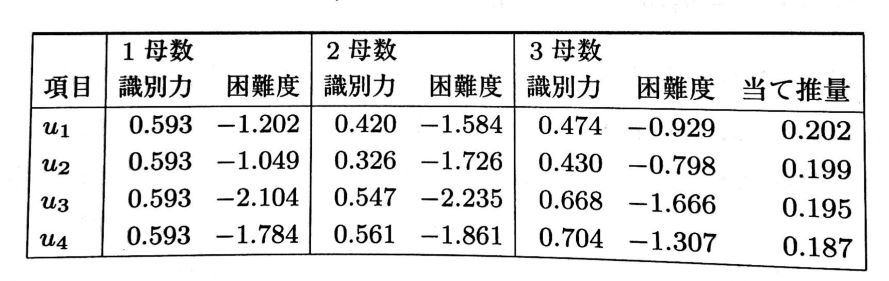
\includegraphics[bb = 0 0 1 1,scale = 0.5]{01.jpg}
\end{figure}
\begin{figure}[H]
  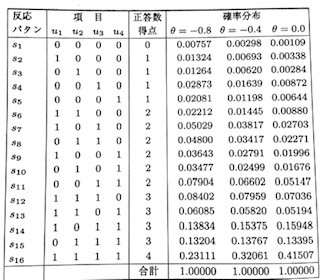
\includegraphics[bb = -3 270 1 1,scale = 1.5]{02.jpg}
\end{figure}



\end{document}
